\chapter{Arquitectura}

\section{Introducción}
En este apartado se describirán la arquitectura del sistema \emph{PushNews}, los diferentes artefactos que lo conforman, la estructura interna de éstos y las tecnologías y frameworks que se han empleado en su construcción.

Como se representa en la figura \ref{fig:diagrama-componentes}, \emph{PushNews} se compone de tres artefactos: una aplicación web, un servicio WEB y una herramienta de monitorización.

\begin{figure}[hb]
  \centering
  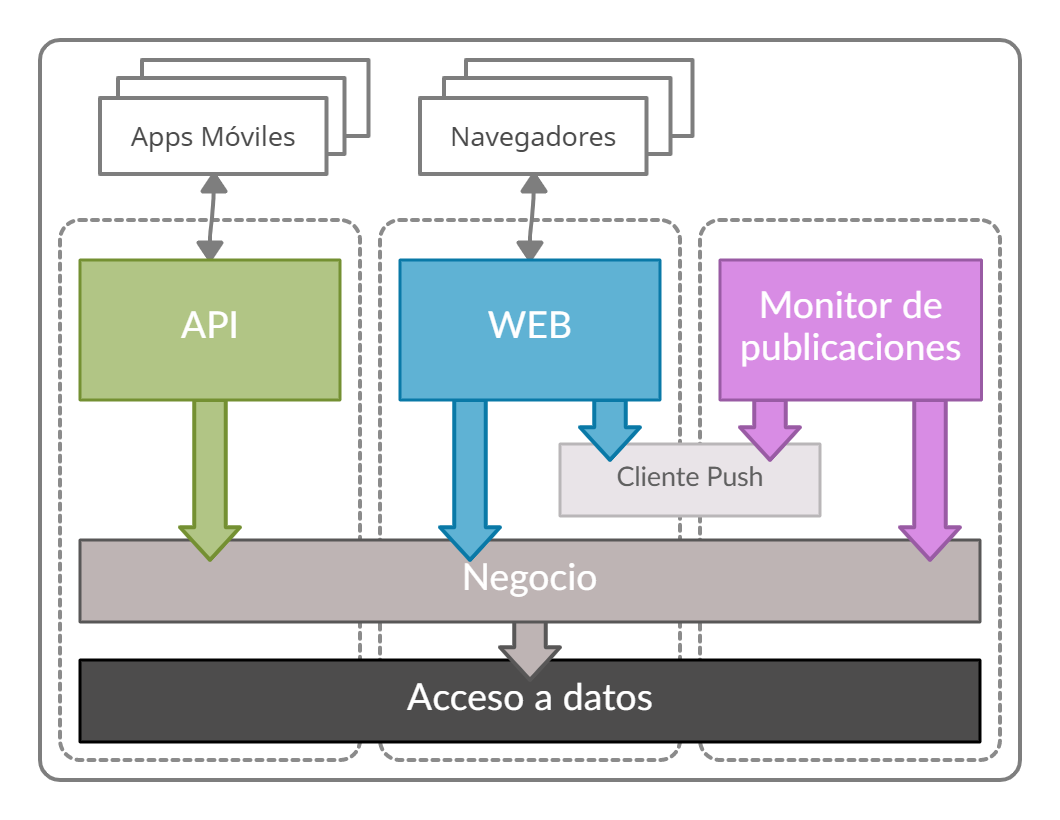
\includegraphics[width=0.8\textwidth]{PushNews Diagrama de componentes}
  \caption{Diagrama de componentes}
  \label{fig:diagrama-componentes}
\end{figure}

\subsection{Capa de acceso a datos}
Explicar el mapeado objeto-relacional, hablar de Entity Framework y mencionar las migraciones.

\section{Patrón MVC}

Modelo-vista-controlador (MVC) es un patrón de arquitectura de software que separa los datos y principalmente lo que es la lógica de negocio de una aplicación de su representación y el módulo encargado de gestionar los eventos y los comunicados. Para ello MVC propone la construcción de tres componentes distintos que son el modelo, la vista y el controlador, es decir, por un lado define componentes para la representación de la información, y por otro lado para la interacción del usuario. Este patrón de arquitectura de software se basa en las ideas de reutilización de código y la separación de conceptos, características que buscan facilitar la tarea de desarrollo de aplicaciones y su posterior mantenimiento \cite{wiki-mvc}.

\begin{figure}[h]
    \centering
    \begin{tikzpicture}[node distance=1cm, auto]
        \tikzset{
            mynode/.style={rectangle,rounded corners,draw=black, top color=white, bottom color=yellow!50,very thick, inner sep=1em, minimum size=3em, text centered},
            myarrow/.style={->, >=latex', shorten >=1pt, thick},
            mylabel/.style={text width=7em, text centered} 
        }
        \node[mynode] (controlador) {Controlador};
        \node[below=3cm of controlador] (dummy) {}; 
        \node[mynode, left=of dummy] (vista) {Vista};
        \node[mynode, right=of dummy] (modelo) {Modelo};
        
        \draw[myarrow] (controlador.south) -- (modelo.north);	
        \draw[myarrow] (vista.north) -- (controlador.south);
        \draw[myarrow] (modelo.west) -- (vista.east);
    \end{tikzpicture}
    \medskip
    \caption{Esquema de la arquitectura Modelo-Vista-Controlador}
\end{figure}